\section{Cahier des charges}
    Un autre objectif de ce projet\footnote{Le premier objectif, qui consiste à effectuer une analyse de la sécurité du réseau STAR, nous servira donc d'exemple pour réaliser ce second objectif.} est de réaliser un outil permettant à un utilisateur (potentiellement novice) d'effectuer une analyse sur la sécurité de son système, quelle qu'en soit sa nature. Cette analyse devra ensuite lui permettre de mettre en place les défenses les plus adaptées et les plus "rentables"\footnote{Rentable en fonction du critère choisi: coût pour l'attaquant, temps pour l'attaquant, difficulté nécessaire pour mener l'attaque, etc.}, jusqu'à obtention d'un système dont la sécurité le satisfait pleinement.
    
    L'analyse reposera grandement sur l'utilisation d'arbres d'attaque--défense, mais aussi sur une expertise (extérieure ou non) qui servira à valuer les feuilles des arbres\footnote{C'est d'ailleurs cette étape qui risque de poser le plus de difficultés à un utilisateur novice.}.
    
    L'outil prendra la forme d'une suite logicielle, dont les différents composants réaliseront chacun une fonctionnalité précise et devront interagir ensemble, et listé ci dessous:
    \begin{itemize}
        \item Une bibliothèque de modèles d'attaques existantes (détaillé dans la sous-section \ref{subsec:biblio_atk}).
        \item Un guide (plus ou moins interactif) pour partir de zéro, même novice (sous-section \ref{subsec:guide_inter}).
        \item Un éditeur d'arbres (sous-section \ref{subsec:edit_arbre}).
    \end{itemize}

    \subsection{Spécifications générales}
        \label{subsec:spec_gen}
        L'analyse de l'utilisateur sera sauvegardée sous forme de projet. Lorsque l'utilisateur voudra faire l'analyse d'un nouveau système, il devra créer un nouveau projet, et répondre à une série de questions, comme par exemple le type du système, l'attaquant envisagé et ses moyens à disposition, et bien d'autres.
        
        Ces informations permettront de présélectionner des modèles plus pertinents au cas de l'utilisateur, et pourront par exemple servir à générer un arbre de base. L'utilisateur pourrait alors l'éditer pour obtenir un arbre d'attaque correspondant à sa situation.

        % Verifier ce que je raconte.
        La valuation des valeurs est déjà prise en charge par ADTool. Toutefois, elle ne permet pas de changer aisement de "type" de valuation. Le projet devrait donc stocker les valeurs des arbres, et pouvoir permettre de changer facilement de valuation (passer du coût au temps, par exemple).
    
    \subsection{Architecture}
        Nous avons décidé de partir sur une architecture modèlaire, où une application mère, qui servira de chef d'orchestre, sera chargé de lancer les différents composants, chacun spécifique à une tache en particulier. % Trop long, reformuler.
        Un ébauche de l'architecture envisagée est disponible figure \ref{fig:archi}.

        \begin{figure}
            \begin{center}
                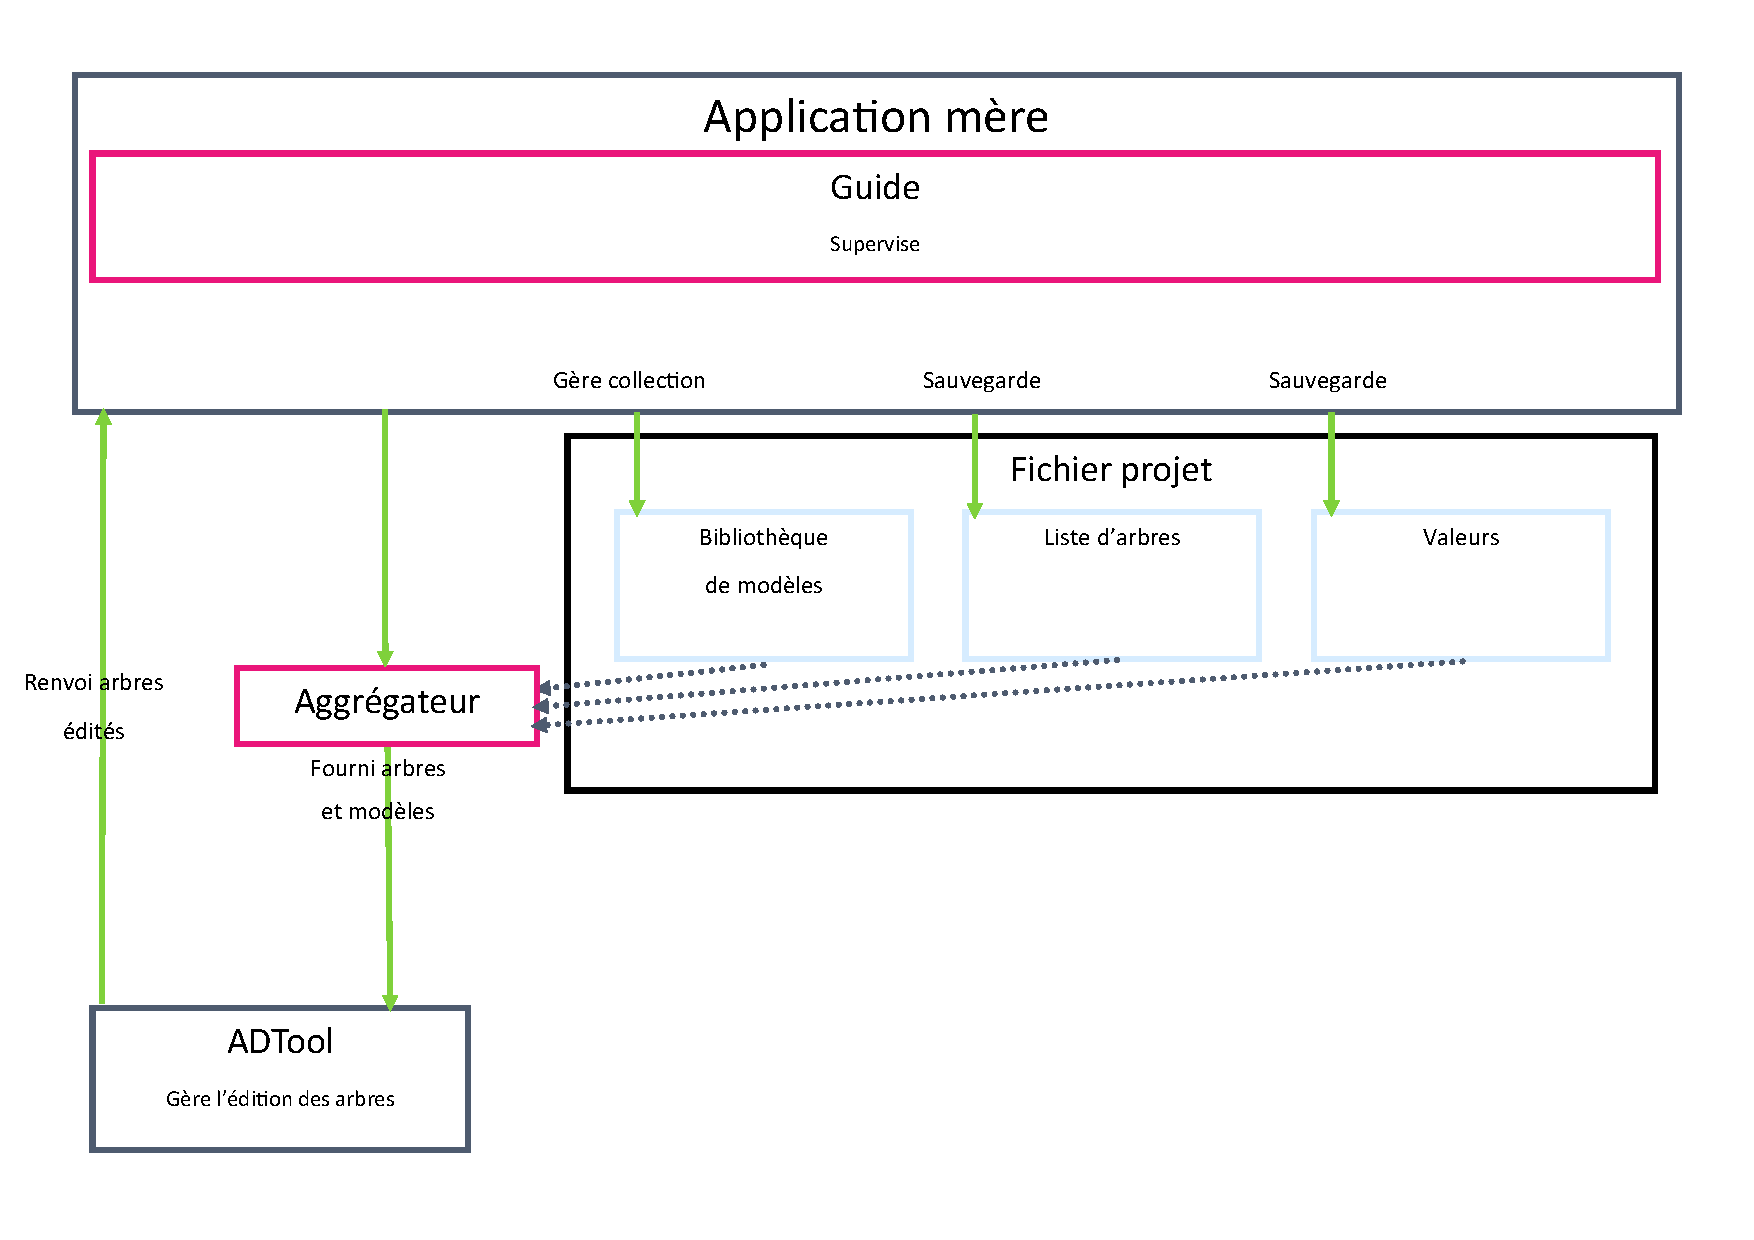
\includegraphics[width=1\textwidth]{figure/archi.pdf}
            \end{center}
            \caption{Différents composants interviendront pour éditer le fichier projet.}
            \label{fig:archi}
        \end{figure}

        % Reformuler ce merdier
        La spécialisation des composants nous permettra d'optenir une architecture logicielle plus propre, qui facilitera le développement: chaque partie sera indépendante des autres, et les choix techniques de l'une ne limiteront pas une autre.

        Avec ce choix d'architecture modulaire, nous réaliserons donc plusieurs outils spécialisés, mais qui le feront bien, plutôt que faire une seule grosse application qui fera tout de manière médiocre et dont l'architecture rendra toute modification très difficile.
        
        De plus, cette architecture peut potentiellement nous permettre de réutiliser certains outils dans d'autres contextes, ou encore de remplacer un des logiciel par un autre sans trop de difficulté. 
    
    \subsection{Bibliothèque d'attaques}  
        \label{subsec:biblio_atk}
        La bibliothèque d'attaques servirait à décrire des cas très généraux, que l'utilisateur pourrait détailler en fonction de sa situation. 
        
        Afin de garder les choses lisibles et ne pas surcharger les autres projets, chaque projet stockera sa propre bibliothèque. De plus, cela rendra la copie de projets entre différents ordinateurs plus aisée.
        
        La bibliothèque d'attaques du projet sera préchargée de diverses attaques en fonction des réponses de l'utilisateur lors de la création du projet, et pourra par la suite être complétée (ou épurée, c'est tout comme) en ajoutant des modèles de base (livrés avec notre application) ou venant d'autres sources (comme Internet, par exemple).
        
        Dans notre exemple (la STAR), nous pourrons fournir des arbres d'attaque de réseaux de transport communs à toutes les villes de France, que nous pourront ensuite détailler pour la ville de Rennes.
      
    \subsection{Guide interactif}
        \label{subsec:guide_inter}
        Le guide doit être capable d'expliquer à l'utilisateur comment faire son analyse. Celle ci sera découpée en plusieurs étapes (en fonction d'une méthode générique que nous auront précédemment présélectionnée).

        Afin de s'adapter à l'expertise de l'utilisateur (allant de novice à expert), son niveau de verbosité pourra être réglé.
        
        Il pourra par exemple poser une série de questions à l'utilisateur, afin de générer un arbre dit "de base" sur lequel l'utilisateur pourra commencer son analyse.
        
        Chaque notion devra être expliquée de manière claire et concise.

        Nous pensions faire référence au célèbre trombone magique de Microsoft Office, mais, pour des raisons de droit, nous utiliseront à la place une agrafeuse.
        
    \subsection{\'Editeur d'arbres}
        \label{subsec:edit_arbre}
        Pour l'édition des arbres, nous utiliserons un outil préexistant, à savoir AD Tool\cite{adtool_paper}.
        
        Toutefois, afin de rendre l'édition des arbres plus simple et plus fluide, nous rajouterons quelques fonctionnalités. Celles ci seront pour la plupart en rapport à l'import/export d'arbres.

        L'objectif en effet serait de faire générer un arbre par notre application mère à partir de différents modèles, pour ensuite demander à l'utilisateur de réaliser les finitions.
    
    \subsection{Multiplateforme}
        Nous allons dans un premier temps nous concentrer sur une seule plateforme, à savoir Microsoft Windows. Ainsi, nous n'auront pas à gérer les difficultés de l'écriture de programmes multi-plateformes, nous laissant le champ libre pour nous occuper uniquement des fonctionnalités de notre application.

        Toutefois, afin de ne pas tuer dans l'oeuf un éventuel portage ultérieur, nous nous éforcerons de choisir des technologies disponibles pour tout les systèmes d'exploitation, afin de minimiser le travail nécessaire.

    \subsection{License}
        Nous souhaitons créer une application open-source, permettant à chacun de reprendre notre projet pour l'améliorer, ou juste prendre certains composants.

        Le choix de la license n'a pas encore été fixé, mais nous risquons de partir sur une GPL. Ceci est dû aux caractéristiques de virus de la GPL.